
\chapterimage{map.png}

\chapter{Arquitectura Empresarial}

\section{Fundamentos de Arquitectura Empresarial}

\subsection{Definición y Propósito}

La Arquitectura Empresarial (AE) es un conjunto integrado de elementos que se utilizan en el diseño y realización de la estructura organizativa, los procesos de negocio, los sistemas de información y la infraestructura de una empresa. Es una práctica estratégica que ayuda a las organizaciones a alinear sus recursos tecnológicos con sus objetivos de negocio.

La AE proporciona:
\begin{itemize}
\item Una visión holística de la organización
\item Un marco para la toma de decisiones estratégicas
\item Una base para la transformación digital
\item Un puente entre la estrategia empresarial y su ejecución
\end{itemize}

\subsection{Beneficios de la Arquitectura Empresarial}

La implementación de una AE ofrece múltiples beneficios:

\begin{itemize}
\item \textbf{Visión común:} Proporciona una visión común de la organización.
\item \textbf{Reducción de complejidad:} Facilita la evolución de los sistemas de información.
\item \textbf{Optimización de costos:} Reduce costos removiendo redundancias.
\item \textbf{Gestión de riesgos:} Reduce riesgos tecnológicos.
\item \textbf{Mejora colaborativa:} Facilita la colaboración entre equipos.
\item \textbf{Alineación estratégica:} Alinea inversiones con objetivos.
\item \textbf{Cumplimiento normativo:} Facilita el cumplimiento regulatorio.
\item \textbf{Resiliencia:} Crea resiliencia organizacional.
\item \textbf{Interoperabilidad:} Garantiza la interoperabilidad del sistema.
\item \textbf{Estandarización:} Estandariza prácticas y procesos.
\end{itemize}



\section{Modelado con ArchiMate}

ArchiMate es el lenguaje de modelado estándar para arquitectura empresarial. Proporciona una forma consistente de visualizar y describir arquitecturas empresariales.

\subsection{Elementos Básicos de ArchiMate}

ArchiMate organiza sus elementos en tres capas principales:
\begin{itemize}
\item \textbf{Capa de Negocio:} Servicios, procesos y actores de negocio
\item \textbf{Capa de Aplicación:} Servicios y componentes de aplicación
\item \textbf{Capa de Tecnología:} Infraestructura y plataformas
\end{itemize}

\subsection{Vistas y Viewpoints}

ArchiMate permite crear diferentes vistas según las necesidades:
\begin{itemize}
\item Vista de Organización
\item Vista de Procesos
\item Vista de Información
\item Vista de Aplicaciones
\item Vista de Infraestructura
\item Vista de Implementación
\end{itemize}

\section{Evaluación de Arquitecturas Empresariales}

La evaluación de arquitecturas empresariales se realiza considerando múltiples dimensiones:

\subsection{Criterios de Evaluación}
\begin{itemize}
\item \textbf{Alineación Estratégica:} ¿La arquitectura soporta los objetivos del negocio?
\item \textbf{Valor del Negocio:} ¿Genera beneficios tangibles?
\item \textbf{Riesgos:} ¿Los riesgos están identificados y gestionados?
\item \textbf{Viabilidad:} ¿Es factible implementar la arquitectura?
\item \textbf{Sostenibilidad:} ¿La arquitectura es mantenible a largo plazo?
\end{itemize}

\subsection{Métricas de Evaluación}
\begin{itemize}
\item Retorno sobre la Inversión (ROI)
\item Tiempo de implementación
\item Costos operativos
\item Nivel de satisfacción de usuarios
\item Cumplimiento regulatorio
\end{itemize}

\section{Caso Práctico: Archisurance}

Manual archi \url{https://www.archimatetool.com/downloads/archi/Archi%20User%20Guide.pdf} 
\\ Caso Archisurance completo \url{https://github.com/archimate-models/archisurance} \\

\begin{tcolorbox}[colback=gray!5!white,colframe=orange!60!gray,title=Archisurance]
Tres compañías de seguros (autos, viajes/casa, legal) ubicadas en diferentes regiones del país, con una buena cartera de clientes, con modelos de negocios similares(seguros), con canales de ventas similares (mediante web, Teléfono y medios postales) han decidido fusionarse. Las razones (drivers) son principalmente pues esto les podría permitir disminuir los costos cuando entran a nuevos mercados, nuevas oportunidades de crecer en otras regiones y la inversión que requieren en TI para mantenerse competitivas puede ser compartido.
\end{tcolorbox}

\subsection{Desarrollo del Caso con Archi}

Para modelar este caso utilizaremos Archi, una herramienta de código abierto para ArchiMate. El proceso incluye:

\subsubsection{Paso 1: Identificación de Stakeholders}
\begin{itemize}
\item Crear nuevo modelo en Archi
\item Identificar stakeholders principales
\item Documentar sus preocupaciones
\end{itemize}

\subsubsection{Paso 2: Análisis de Motivación}
\begin{itemize}
\item Crear vista de motivación
\item Identificar drivers del negocio
\item Establecer metas y objetivos
\end{itemize}

\begin{figure}[h]
\centering
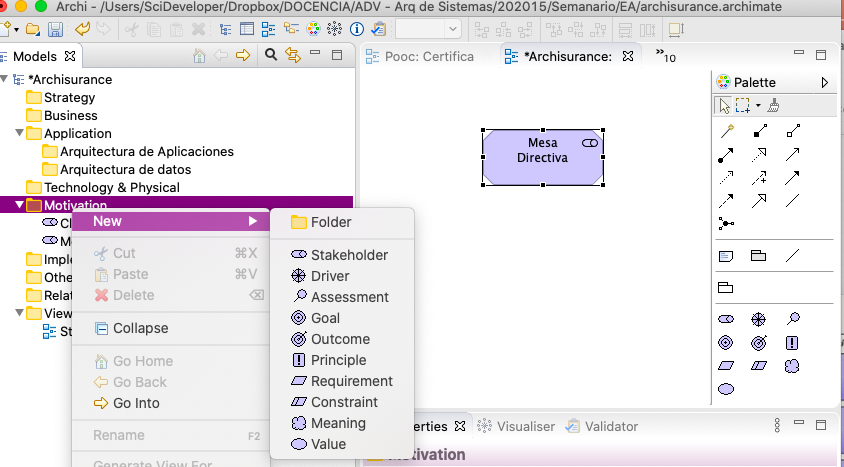
\includegraphics[scale=0.35]{Pictures/addstake.png}
\caption{Agregando stakeholders en Archi.}
\label{fig:stakeholders}
\end{figure}

\subsubsection{Paso 3: Modelado de Arquitectura}
\begin{itemize}
\item Desarrollar vista de negocio
\item Crear vista de aplicaciones
\item Diseñar vista de tecnología
\end{itemize}

\begin{figure}[h]
\centering
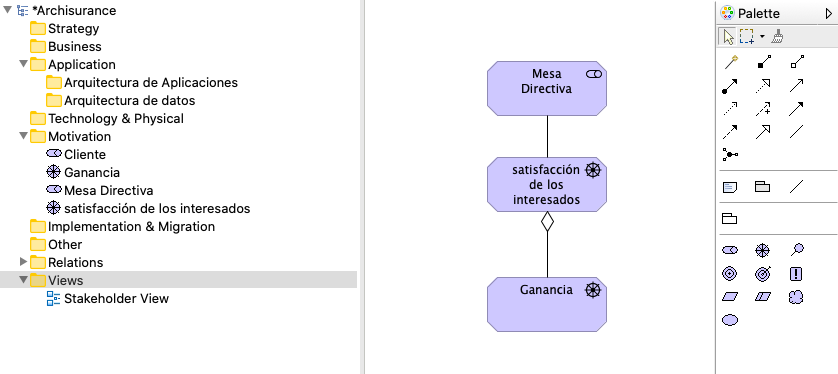
\includegraphics[scale=0.35]{Pictures/jeraquiadrivers.png}
\caption{Jerarquía de drivers en Archi.}
\label{fig:drivers}
\end{figure}




\section{Marco de Referencia TOGAF}

\subsection{Introducción a TOGAF}

The Open Group Architecture Framework (TOGAF) es un marco reconocido globalmente para el desarrollo y la gestión de arquitecturas empresariales. Diseñado para arquitectos empresariales y responsables de arquitectura en organizaciones, TOGAF ofrece un enfoque estructurado y flexible.

Inicialmente desarrollado en 1995, basado en el Marco de Arquitectura Técnica para la Gestión de la Información (TAFIM) del Departamento de Defensa de los Estados Unidos, TOGAF ha evolucionado para adaptarse a las necesidades modernas. Permite a las organizaciones optimizar su estructura para responder al cambio y respaldar estrategias empresariales.

\begin{figure}[h]
\centering
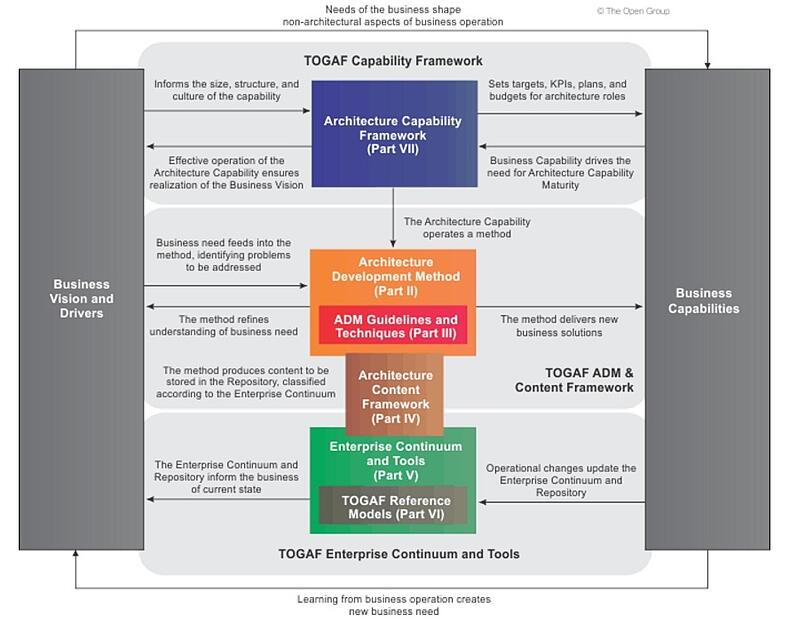
\includegraphics[scale=0.6]{Pictures/togaf.jpg}
\caption{Estructura del estándar TOGAF.}
\label{fig:togaf_structure}
\end{figure}

\subsection{Dominios de la Arquitectura Empresarial}

La AE se divide en cuatro dominios principales que trabajan de manera integrada:

\subsubsection{Arquitectura de Negocio}
Define la estrategia del negocio, la gobernanza, la estructura y los procesos clave. Incluye:
\begin{itemize}
\item Procesos de negocio
\item Estructura organizacional
\item Objetivos y metas estratégicas
\item Servicios de negocio
\item Métricas de rendimiento
\end{itemize}

\subsubsection{Arquitectura de Datos}
Describe la estructura de los datos lógicos y físicos de la organización:
\begin{itemize}
\item Modelos de datos
\item Políticas de gestión de datos
\item Estándares de datos
\item Flujos de información
\item Calidad y gobierno de datos
\end{itemize}

\subsubsection{Arquitectura de Aplicaciones}
Define las aplicaciones necesarias para procesar los datos y soportar las funciones del negocio:
\begin{itemize}
\item Catálogo de aplicaciones
\item Interfaces entre aplicaciones
\item Ciclos de vida de las aplicaciones
\item Patrones de arquitectura
\item Integración de sistemas
\end{itemize}

\subsubsection{Arquitectura Tecnológica}
Describe la infraestructura de hardware y software que soporta las aplicaciones y datos:
\begin{itemize}
\item Infraestructura de TI
\item Redes y comunicaciones
\item Procesamiento y almacenamiento
\item Estándares tecnológicos
\item Seguridad tecnológica
\end{itemize}

\section{Método de Desarrollo de Arquitectura (ADM)}

El ADM de TOGAF es un método iterativo que guía el desarrollo de la arquitectura empresarial a través de un ciclo continuo de definición y realización de arquitectura.

\subsection{Fases del ADM}
\begin{itemize}
\item \textbf{Fase Preliminar:} Preparación e iniciación. Establece las capacidades arquitectónicas iniciales.
\item \textbf{Fase A:} Visión de Arquitectura. Define el alcance, limitaciones y expectativas del proyecto arquitectónico.
\item \textbf{Fase B:} Arquitectura de Negocio. Desarrolla la arquitectura de negocio para apoyar la visión acordada.
\item \textbf{Fase C:} Arquitectura de Sistemas de Información. Desarrolla las arquitecturas de datos y aplicaciones.
\item \textbf{Fase D:} Arquitectura Tecnológica. Define la infraestructura necesaria para soportar la arquitectura objetivo.
\item \textbf{Fase E:} Oportunidades y Soluciones. Identifica los principales proyectos de implementación.
\item \textbf{Fase F:} Planificación de Migración. Desarrolla el plan detallado de implementación y migración.
\item \textbf{Fase G:} Gobierno de Implementación. Supervisa la implementación para asegurar conformidad.
\item \textbf{Fase H:} Gestión de Cambios en la Arquitectura. Monitorea y gestiona los cambios.
\end{itemize}

\subsection{Componentes Clave del ADM}
\begin{itemize}
\item \textbf{Entregables:} Son los productos de trabajo formalmente revisados, acordados y firmados por los stakeholders. Incluyen:
  \begin{itemize}
    \item Documentos de definición de arquitectura
    \item Especificaciones de requerimientos
    \item Planes de implementación y migración
    \item Evaluaciones de cumplimiento
  \end{itemize}

\item \textbf{Artefactos:} Son los productos de trabajo específicos que describen un aspecto de la arquitectura:
  \begin{itemize}
    \item Catálogos: Listas de bloques de construcción
    \item Matrices: Muestran relaciones entre componentes
    \item Diagramas: Representaciones gráficas de la arquitectura
  \end{itemize}

\item \textbf{Bloques de Construcción:} Representan componentes reutilizables que:
  \begin{itemize}
    \item Pueden ser combinados para entregar arquitecturas y soluciones
    \item Proporcionan capacidades que resuelven necesidades del negocio
    \item Son reutilizables y configurables según el contexto
  \end{itemize}
\end{itemize}

\subsection{Aplicación del ADM: Caso DART-MINSAL}

Para ilustrar la aplicación práctica del ADM, analizaremos el caso del sistema DART (Detección Automatizada de Retinopatía Diabética) del MINSAL:

\subsubsection{Fase Preliminar}
\begin{itemize}
\item \textbf{Contexto:} Sistema de salud chileno con déficit de 39,168 horas de atención oftalmológica
\item \textbf{Principios:} 
  \begin{itemize}
    \item Acceso equitativo a servicios de salud
    \item Optimización de recursos médicos
    \item Transformación digital en salud pública
  \end{itemize}
\end{itemize}

\subsubsection{Fase A: Visión de Arquitectura}
\begin{itemize}
\item \textbf{Objetivos Estratégicos:}
  \begin{itemize}
    \item Reducir tiempo de diagnóstico de 30 a 5 días
    \item Optimizar uso de oftalmólogos (de 39,168 a 15,000 horas/año)
    \item Aumentar cobertura en zonas rurales de 40\% a 90\%
  \end{itemize}
\item \textbf{Balance Scorecard:}
  \begin{itemize}
    \item Perspectiva Financiera: Reducción de costos en diagnósticos
    \item Perspectiva Cliente: Garantizar acceso oportuno a servicios
    \item Perspectiva Procesos: Reducir brechas en zonas rurales
    \item Perspectiva Aprendizaje: Prevenir enfermedades crónicas
  \end{itemize}
\end{itemize}

\subsubsection{Fase B: Arquitectura de Negocio}
\begin{itemize}
\item \textbf{Procesos Clave:}
  \begin{itemize}
    \item Preprocesar imágenes
    \item Detectar signos de retinopatía
    \item Generar propuesta de reporte
    \item Validación profesional
    \item Notificar paciente
  \end{itemize}
\item \textbf{Actores:} MinSal, Oftalmólogos, Pacientes diabéticos
\end{itemize}

\subsubsection{Fase C: Arquitectura de Sistemas de Información}
\begin{itemize}
\item \textbf{Arquitectura de Datos:}
  \begin{itemize}
    \item Datos de Ficha Clínica
    \item Imágenes de Retina
    \item Datos de Informes Médicos
  \end{itemize}
\item \textbf{Arquitectura de Aplicaciones:}
  \begin{itemize}
    \item DART Connector
    \item CRM
    \item Notifier
    \item DataTransformer
  \end{itemize}
\end{itemize}

\subsubsection{Fase D: Arquitectura Tecnológica}
\begin{itemize}
\item \textbf{Infraestructura Hospital:}
  \begin{itemize}
    \item Servidor de Telemedicina
    \item Servidor de Imagenología
    \item Conector DART
  \end{itemize}
\item \textbf{Infraestructura Nube:}
  \begin{itemize}
    \item Servidor de Procesamiento IA
    \item Repositorio de Diagnósticos
    \item API Gateway del MINSAL
  \end{itemize}
\item \textbf{Seguridad:}
  \begin{itemize}
    \item Cifrado de datos
    \item VPN/Canales Seguros
    \item Autenticación entre sistemas
  \end{itemize}
\end{itemize}

\subsubsection{Fase E: Oportunidades y Soluciones}
\begin{itemize}
\item \textbf{Proyectos Identificados:}
  \begin{itemize}
    \item Implementación de DART en hospitales
    \item Automatización del cribado con IA
    \item Expansión de estaciones de diagnóstico
    \item Integración con ficha clínica electrónica
  \end{itemize}
\end{itemize}

\subsubsection{Fase F: Plan de Migración}
\begin{itemize}
\item \textbf{Métricas Clave:}
  \begin{itemize}
    \item Tiempo promedio de diagnóstico
    \item Horas oftalmológicas utilizadas
    \item Cobertura de exámenes en APS rurales
    \item Nivel de digitalización de procesos
  \end{itemize}
\item \textbf{Metas a 5 Años:}
  \begin{itemize}
    \item Reducir tiempo de diagnóstico a 5 días
    \item Optimizar a 15,000 horas/año de oftalmólogos
    \item Alcanzar 90\% de cobertura rural
    \item Lograr 95\% de digitalización
  \end{itemize}
\end{itemize}

\begin{figure}[h]
\centering
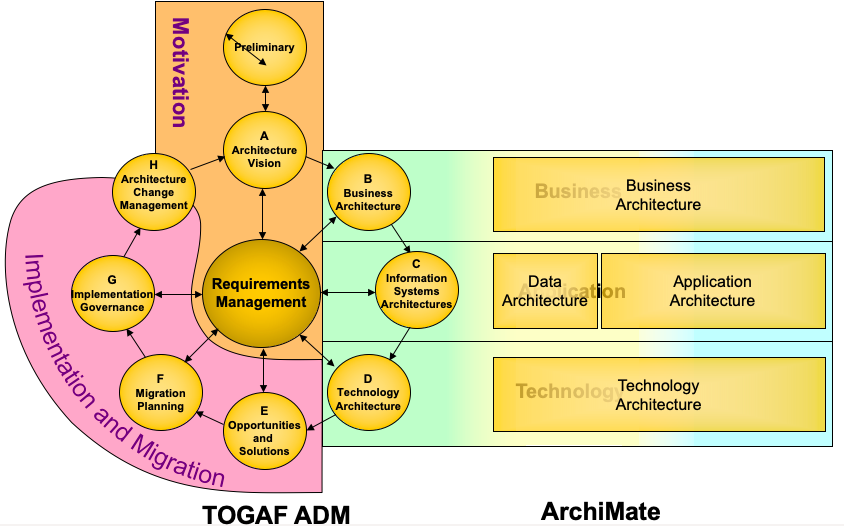
\includegraphics[scale=0.6]{Pictures/ADM.png}
\caption{Ciclo del Método de Desarrollo de Arquitectura (ADM).}
\label{fig:adm_phases}
\end{figure}




\section{Recursos y Referencias}

Para profundizar en el uso de Archi y ArchiMate:

\begin{itemize}
\item Manual Archi: \url{https://www.archimatetool.com/downloads/Archi\%20User\%20Guide.pdf}
\item Especificación ArchiMate: \url{https://pubs.opengroup.org/architecture/archimate3-doc/toc.html}
\item Caso Archisurance completo: \url{https://publications.opengroup.org/y163}
\end{itemize}



